\begin{figure}[H]
\centering
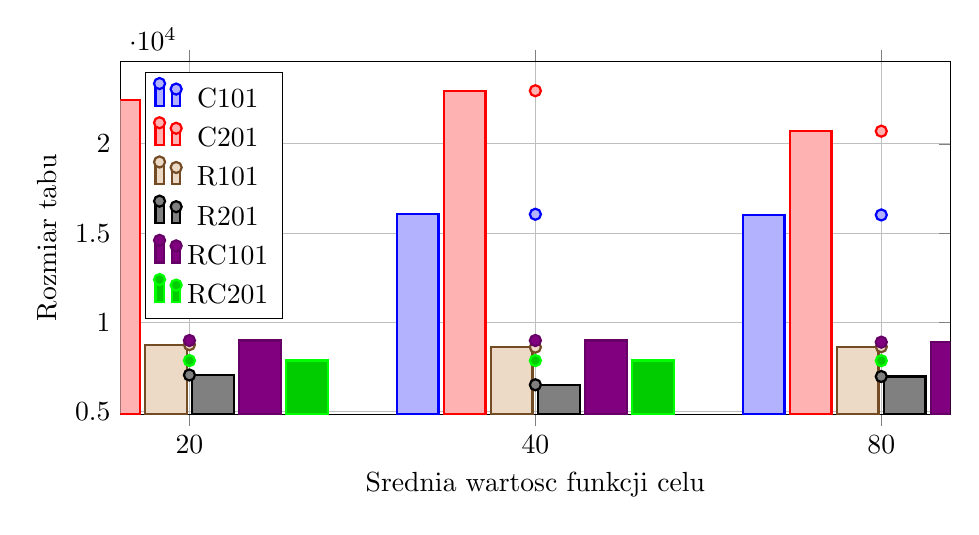
\begin{tikzpicture}
\begin{axis}[
xlabel = {Srednia wartosc funkcji celu},
ylabel = {Rozmiar tabu},
legend pos = north west,
grid = both,
width=1\linewidth,
height=0.5\linewidth,
ybar,
bar width=15pt,
symbolic x coords={20,40,80,},
xtick=data
]
\addplot + [mark = *, thick] coordinates
    {
(20,16057.75)(40,16057.75)(80,16019.5)};
\addlegendentry
{C101}
\addplot + [mark = *, thick] coordinates
    {
(20,22477.25)(40,22977.0)(80,20711.0)};
\addlegendentry
{C201}
\addplot + [mark = *, thick] coordinates
    {
(20,8750.75)(40,8611.25)(80,8636.25)};
\addlegendentry
{R101}
\addplot + [mark = *, thick] coordinates
    {
(20,7053.5)(40,6505.25)(80,6969.25)};
\addlegendentry
{R201}
\addplot + [mark = *, thick] coordinates
    {
(20,8985.0)(40,8985.0)(80,8893.0)};
\addlegendentry
{RC101}
\addplot + [mark = *, thick] coordinates
    {
(20,7861.0)(40,7861.5)(80,7855.25)};
\addlegendentry
{RC201}
\end{axis}
\end{tikzpicture}
\caption
{Srednia wartosc funkcji celu w zaleznosci od rozmiaru tabu dla poszczegolnych instancji}
\label{fig:mean_goals_per_tabu_size_per_instance}
\end{figure}
